\newcommand{\AWSSTS}{Serviciu web ce permite unui utilizator să solicite credențiale temporare pentru autentificarea în cadrul platformei Amazon Web Services}
\newcommand{\openIDDefinition}{http://openid.net/what-is-openid/}

\usemintedstyle{rrt}

Esența aplicației "Surf" se află în codul executat de serviciul web AWS Lambda, care preia componentele dezvoltate pentru crawling web și le execută, drept programe autonome, folosind infrastructura AWS. AWS Lambda execută acest cod doar când este nevoie (e.g. la cererea utilizatorului care dorește să demareze operațiunea de crawling). Se minimizează, astfel, atât costurile utilizatorului în ceea ce privește rularea crawler-ului web (nu necesită hardware dedicat pentru procesarea paginilor web), cât și costurile dezvoltatorilor crawler-ului, care nu trebuie să rezerve hardware în cloud (e.g. mașini virtuale Amazon EC2, închiriere de mașini gazdă), ca, mai apoi, când nu există cereri suficiente, aceste mașini de calcul să ramână nefolosite. De asemenea, se renunță la necesitatea de a avea un load-balancer care să distribuie sarcinile de crawling pe capacitatea hardware disponibilă, deoarece acest lucru este administrat, în fundal, de catre AWS Lambda.
\\
\\
Funcțiile programatice disponibile prin serviciul AWS Lambda pot fi accesate de către utilizatori printr-un API Restful, găzduit de AWS API Gateway. Această platformă permite integrarea cererilor HTTP externe cu mecanismul de autentificare și autorizare a utilizatorilor și codul executat de insțantele funcțiilor Lambda. De asemenea, aplicația utilizează funcționalități de management, monitorizare și analiză a traficului din cadrul API-ului "Surf" care permit, printre altele, înregistrarea și monetizarea funcționalitatilor oferite de serviciul web pentru fiecare utilizator în parte. 
\\
\\
Pentru a putea accesa funcționalitățile oferite de API-ul "Surf", utilizatorii trebuie să se autentifice cu un furnizor terț de identități OpenID\footnote{\openIDDefinition}. Credențialele obținute sunt împachetate într-o cerere catre AWS Security Token Service\footnote{\AWSSTS}, unde sunt validate. În cazul în care validarea este îndeplinită cu succes, Security Token Service returnează utilizatorului credențiale temporare pentru a accesa servicii din cadrul AWS. Utilizatorul trebuie să includă aceste credențiale în fiecare cerere catre API-ul "Surf" (autentificare). Odată autentificat, utilizatorul poate interacționa doar cu acele resurse ale API-ului pentru care are drepturi de acces. 

\begin{figure}[ht]
\begin{center}
	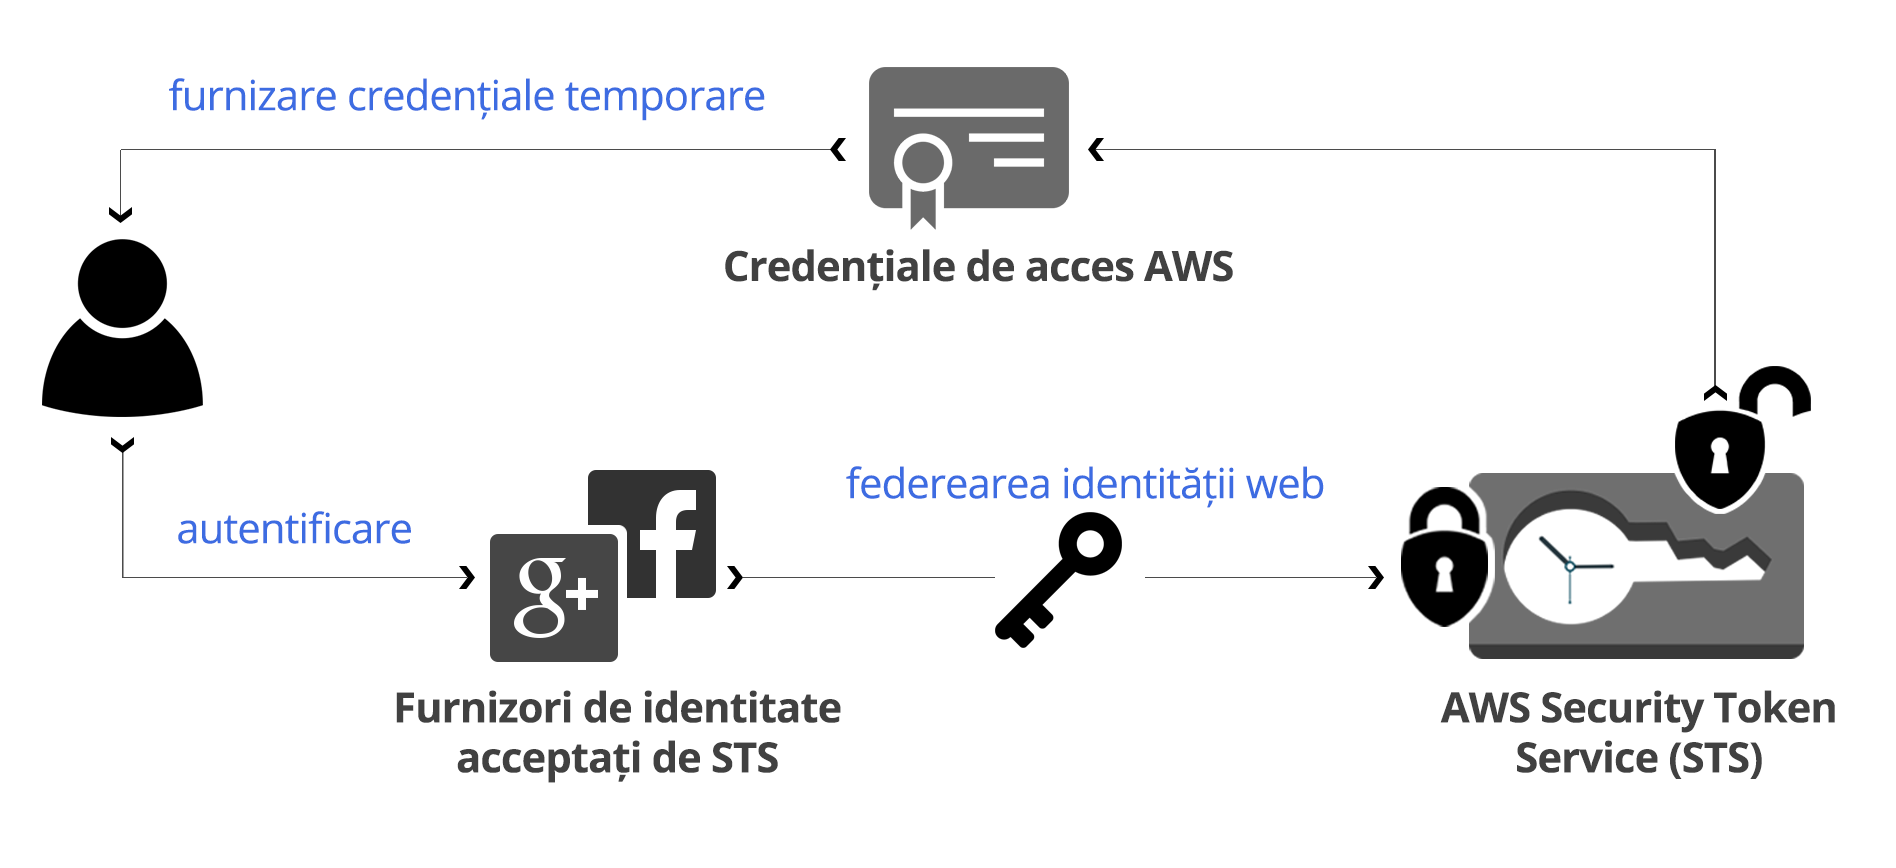
\includegraphics[keepaspectratio, width=1.0\textwidth]{obtinere-credentiale-aws.png}
	\caption{Procesul de autentificare \cite{diagram-icons-sources}}\par\medskip
	\vspace{10mm}
	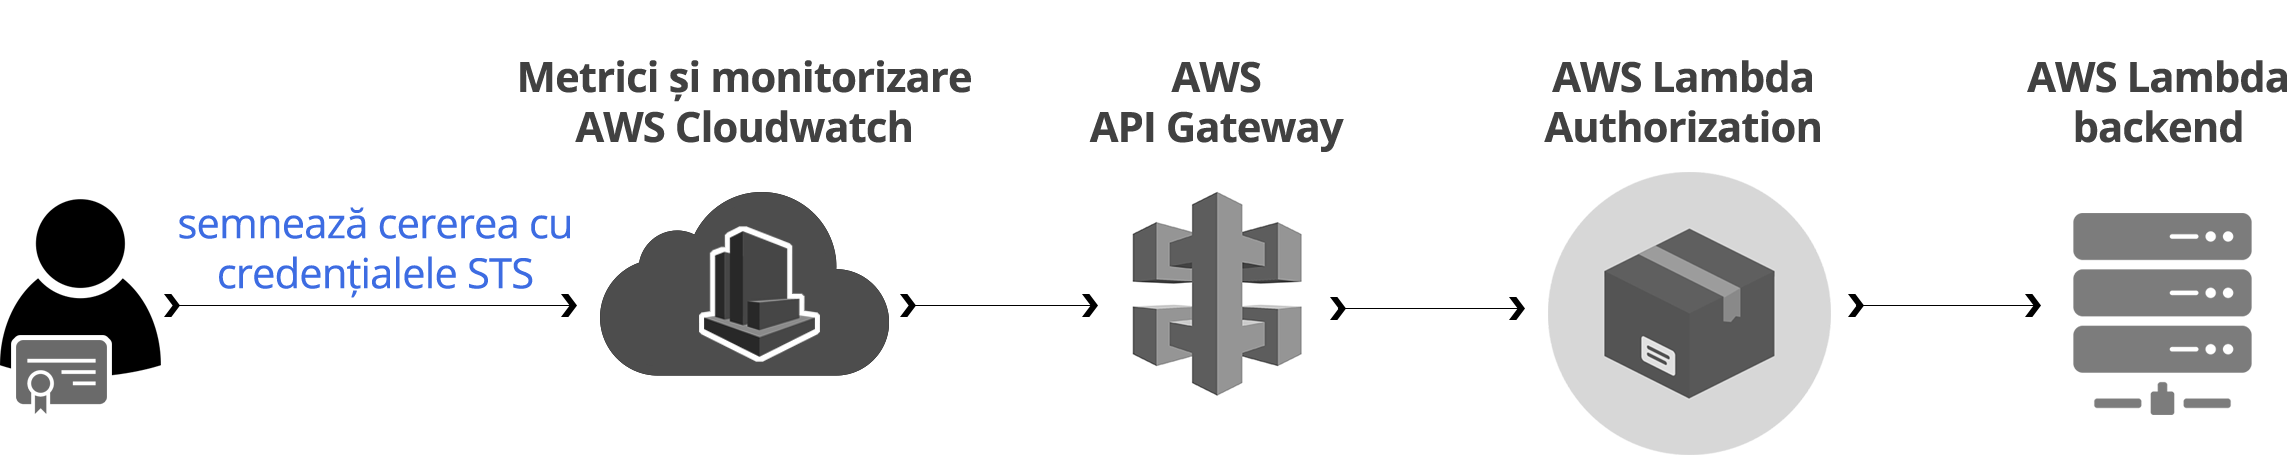
\includegraphics[keepaspectratio, width=1.0\textwidth]{autorizare.png}
	\caption{Procesul de autorizare \cite{diagram-icons-sources}}\par\medskip

\end{center}
\end{figure}

\noindent
Prin AWS Identity Access Management (IAM) se vor stabili restricțiile de acces asupra API-ului. Mecanismul de asignare a permisiunilor va fi susținut prin definirea unor roluri. Utilizatorii vor fi grupați, din punct de vedere al drepturilor de acces, în mai multe categorii. Spre exemplu, un utilizator poate avea rolul "administrator" (prescurtat \emph{Ad}), iar un alt utilizator poate avea atât rolul "administrator" (\emph{Ad}), cât și "utilizator de bază" (prescurtat \emph{Ub}). Atât \emph{Ad}, cât și \emph{Ub} vor avea asignate politici de acces asupra datelor AWS. O astfel de politică este următoarea:

\begin{figure}[ht]
\begin{minted}[fontsize=\footnotesize]{json}
{
  "Version": "2012-10-17", // Stabilită de către furnizor
  "Statement": [
    {
      "Effect": "Allow",
      "Action": [
        "apigateway:*"
      ],
      "Resource": [
        "*"
      ]
    }
  ]
}
\end{minted}
\begin{center}
	\caption{Politică de acces IAM}\par\medskip
\end{center}
\end{figure}

\noindent
Politica de acces de mai sus îi permite utilizatorului ce îi este asignată accesul la toate resursele API-ului "Surf". Această politică este potrivită pentru un administrator, dar periculoasă pentru un utilizator ce accesează pentru prima data serviciul "Surf". De aceea, se vor defini drepturi de acces granulare care să aibă în vedere restricționarea la nivel "need-to-know"\footnote{http://dictionary.cambridge.org/dictionary/english/on-a-need-to-know-basis} pentru fiecare entitate ce trimite cereri către API (autorizare).
\\
\\
Procesul de asignare a rolurilor pentru utilizatori este coordonat atât manual (pe bază de ierarhie: administrator - utilizator de baza), cât și automat (i.e. printre altele, toți utilizatorii abia înregistrați sunt utilizatori standard). Asignarea manuală a permisiunilor are prioritate asupra asignării automate. Datele despre rolul fiecărui utilizator vor fi păstrate în baza de date.
\\

\noindent
Crawler-ul "Surf" utilizează AWS DynamoDB ca suport pentru baza de date. DynamoDB reprezintă un serviciu cloud scalabil pentru baze de date NoSQL. Datele dintr-o bază de date non-relațională NoSQL) pot fi modelate fără constrângerile unei baze de date relaționale (e.g. tabularitate). Acest lucru atrage, în cadrul aplicației "Surf", elemente operaționale cheie, pentru beneficiul cărora s-a renunțat la o abordare relațională, de tip SQL (e.g. Oracle), printre care:


\begin{itemize}

	\item{\emph{data sharding}\footnote{https://docs.microsoft.com/en-us/azure/architecture/patterns/sharding} - este necesar un sistem distribuit de baze de date care să poată scala orizontal odată cu dimensiunea datelor din baza de date și odată cu creșterea numărului de utilizatori;}
	\item{\emph{scheme de date dinamice}\footnote{https://www.mongodb.com/scale/dynamic-schema-design} - se dorește posibilitatea schimbării structurii datelor din baza de date fără a recrea tabelele corespunzătoare; acest lucru trebuie avut în vedere deoarece crawler-ul stochează în baza de date metadate obținute prin parcurgerea paginilor web; poate apărea oricând necesitatea introducerii unor noi metadate sau schimbării structurii celor existente, cu scopul satisfacerii nevoilor utilizatorilor.}
	
\end{itemize}

\noindent
Câteva dintre cele mai importante roluri ale bazei de date sunt găzduirea metadatelor asociate rezultatelor procesului de crawling, păstrarea asignărilor între identitățile utilizatorilor și rolurile lor, menținerea istoricului evenimentelor de crawling cu scopul reconstruirii stării procesului de parcurgere a paginilor web, în cazul unei erori, și stocarea datelor asociate volumului de trafic generat de fiecare utilizator în cadrul infrastructurii AWS.
\\
\\
Pentru a obține un serviciu web distribuit pentru crawling este necesară coordonarea activităților independente din cadrul sistemului, sincronizarea pașilor necesari procesului de crawling și, în final, integrarea rezultatelor. Pentru acest lucru, aplicația "Surf" folosește serviciul web AWS Step Functions (SFN). SFN  are capacități de coordonare a activităților ce se doresc îndeplinite (i.e. execuția funcțiilor Lambda, sau \emph{Lambda Tasks}) și management al stării aplicației (i.e. se pornește un proces de agregare a datelor provenite de la crawlerii care au rulat în paralel doar după ce aceștia și-au terminat execuția).
\\
\\
Datele obținute în urma procesului de crawling sunt stocate utilizând serviciul web Amazon S3. Fiecare rulare a unei instanțe a crawler-ului distribuit generează un \emph{bucket}\footnote{Unitate, în cloud (AWS S3), ce stochează date și căreia îi pot fi atribuite permisiuni de acces și metadate corespunzatoare} S3. Datele din bucket-uri sunt disponibile, pentru utilizatori, prin plasarea de metadate, precum numele bucket-ului, într-o tabelă DynamoDB, pe care utilizatorii o pot accesa prin intermediul API-ului.

